\documentclass[border=10pt]{standalone}

\usepackage{tikz}
\usepackage{tikzsymbols}
\usetikzlibrary{calc,patterns,shapes.geometric}

\def\centerarc[#1](#2)(#3:#4:#5){\draw[#1] ($(#2)+({#5*cos(#3)},{#5*sin(#3)})$) arc (#3:#4:#5);}

\begin{document}
	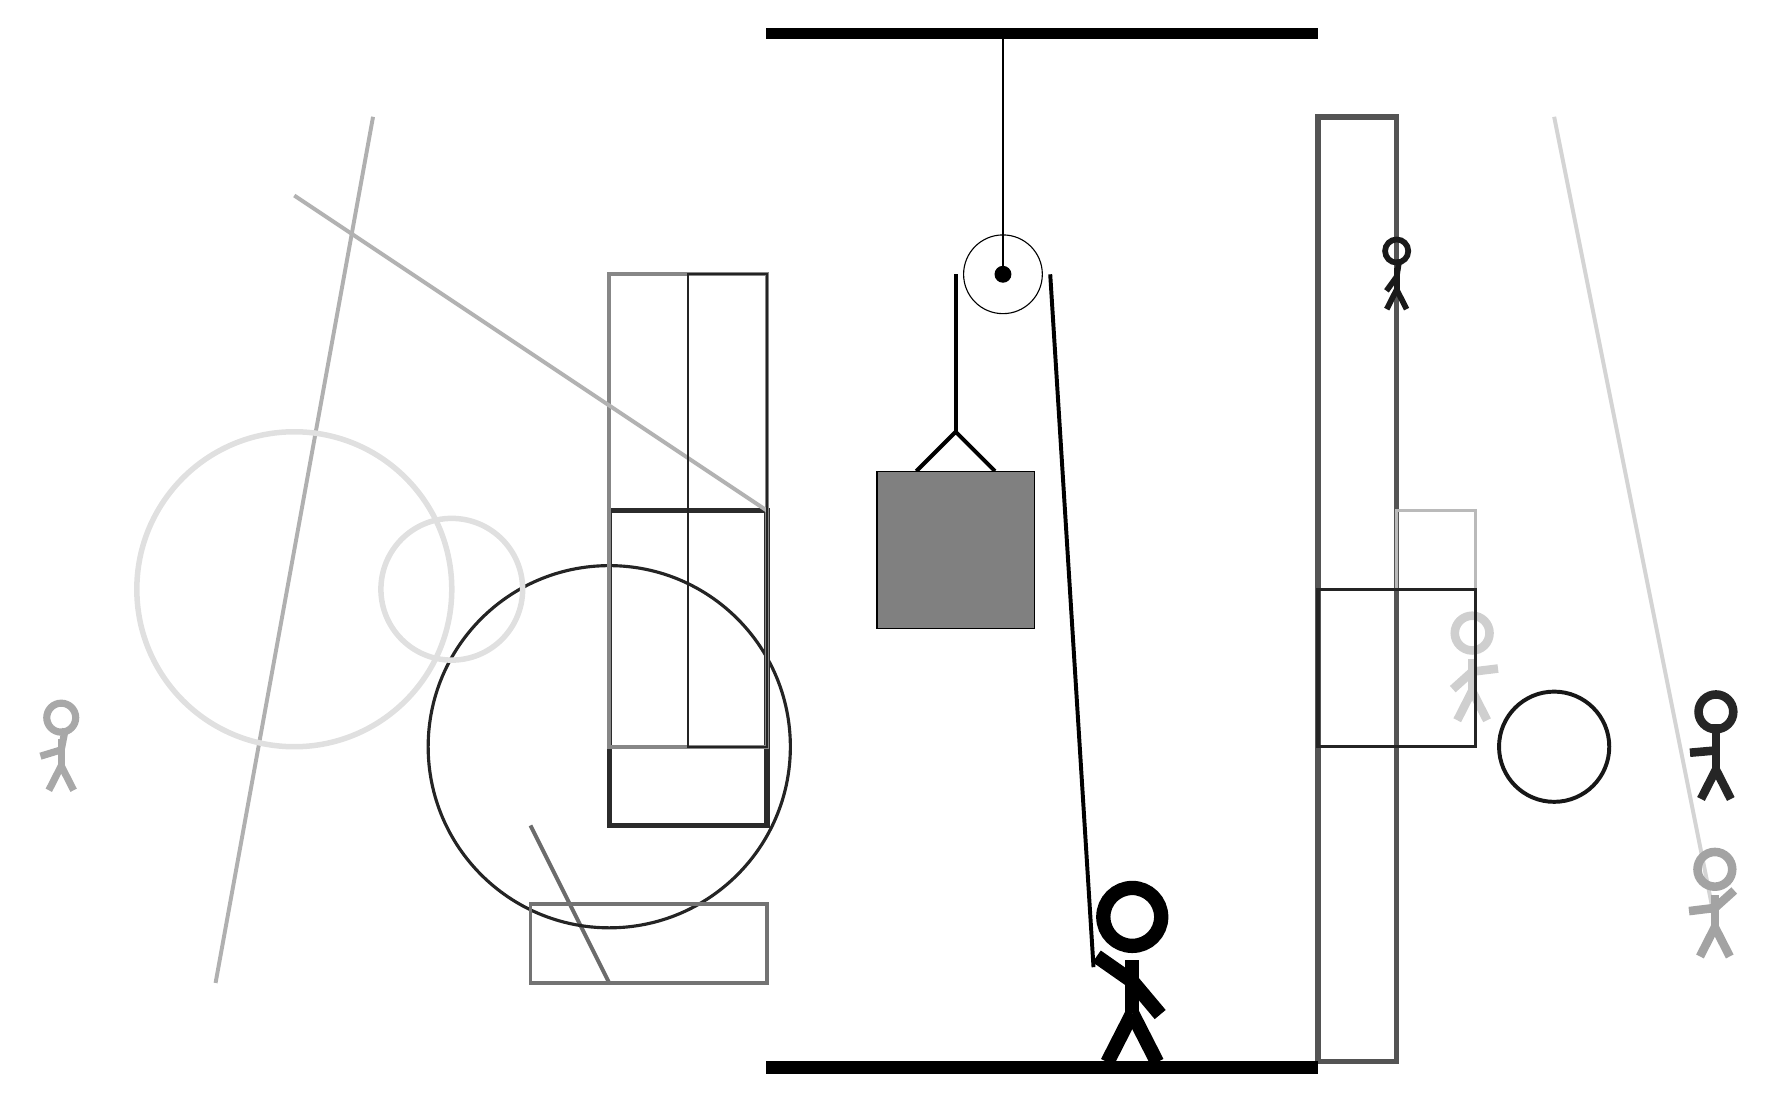
\begin{tikzpicture}
		%%%%% START %%%%%
		
		\draw[fill=black] (-2, 10) rectangle (5, 10.125);
		
		\draw[line width=0.5mm, color=black!27](-7, 4) -- (-7, 4);
		
		\node[line width=0.4mm, color=black!34] at (-11, 1) {\Strichmaxerl[5][17][79]};
		\draw[line width=0.5mm, color=black!17](8, 9) -- (10, -1);
		\draw [line width=0.4mm, color=black!84](-6, 6) circle (0.0);
		
		\draw[line width=0.7mm, color=black!67] (6, -3) rectangle (5, 9);
		\draw[line width=0.5mm, color=black!31](-7, 9) -- (-9, -2);
		
		\draw[line width=0.5mm, color=black!58](-4, -2) -- (-5, 0);
		\draw [line width=0.4mm, color=black!86](-4, 1) circle (2.3);
		\draw[line width=0.7mm, color=black!83] (-2, 4) rectangle (-4, 0);
		\draw[line width=0.5mm, color=black!47] (-4, 7) rectangle (-2, 1);
		\draw[line width=0.4mm, color=black!27] (6, 4) rectangle (7, 3);
		\draw [line width=0.7mm, color=black!12](-8, 3) circle (2.0);
		\draw[line width=0.5mm, color=black!30](-2, 4) -- (-8, 8);
		
		\draw [line width=0.5mm, color=black!34](-2, 3) circle (0.0);
		\draw[line width=0.5mm, color=black!55] (-2, -1) rectangle (-5, -2);
		\draw[line width=0.3mm, color=black!86] (-2, 7) rectangle (-3, 1);
		
		\node[line width=0.4mm, color=black!36] at (10, -1) {\Strichmaxerl[6][7][42]};
		
		\node[line width=0.5mm, color=black!19] at (7, 2) {\Strichmaxerl[6][42][7]};
		\draw [line width=0.5mm, color=black!91](8, 1) circle (0.7);
		\node[line width=0.6mm, color=black!90] at (6, 7) {\Strichmaxerl[4][54][81]};
		\draw [line width=0.7mm, color=black!12](-6, 3) circle (0.9);
		
		\node[line width=0.5mm, color=black!85] at (10, 1) {\Strichmaxerl[6][5][90]};
		
		\draw[line width=0.4mm, color=black!86] (5, 3) rectangle (7, 1);
		
		\draw (1, 7) circle (0.5);
		\draw[fill=black] (1, 7) circle (0.1);
		\draw (1, 10) -- (1, 7);
		
		\draw[line width=0.5mm] (-0.1, 4.5) -- (0.4, 5.0) -- (0.9, 4.5);
		\draw[fill=black!50] (-0.6, 4.5) rectangle (1.4, 2.5);
		
		\draw[line width=0.5mm] (0.4, 7) -- (0.4, 5.0);
		\centerarc[line width=0.5mm](1, 7)(0:180:0.6);
		\draw[line width=0.5mm](1.6, 7) -- (2.15, -1.8);
		
		\node at (2.6, -1.9) {\Strichmaxerl[10][-35][-50]};
		
		\draw[fill=black] (-2, -3) rectangle (5, -3.15);
		
		%%%%% END %%%%%
	\end{tikzpicture}
\end{document}